\section{Experimental Evaluation}

We evaluate the performance of our SEM-SpMM on multiple real-world billion-scale
graphs including a web-page graph with 3.4 billion vertices. We first measure
the performance of SEM-SpMM and compare it with our in-memory implementation
(IM-SpMM), which is simply the SEM-SpMM implementation with the sparse matrix
in memory.
We also compare SEM-SpMM with state-of-the-art in-memory implementations in
Intel MKL (\textit{mkl\_dcsrmm}) and Trilinos Tpetra. We use Intel MKL 2015
and Trilinos v12.0.1 for the experiments. We demonstrate the effectiveness of
CPU and I/O optimizations on SEM-SpMM and evaluate the overall performance
of the applications in Section \ref{sec:spmm:apps}.

We conduct experiments on a non-uniform memory architecture machine with
four Intel Xeon E7-4860 processors, clocked at 2.6 GHz, and 1TB memory of
DDR3-1600. Each processor has 12 cores. The machine has three LSI SAS 9300-8e
host bus adapters (HBA) connected to a SuperMicro storage chassis, in which
24 OCZ Intrepid 3000 SSDs are installed. The 24 SSDs together are capable of
delivering 12 GB/s for read and 10 GB/s for write at maximum. The machine runs
Linux kernel v3.13.0. We use 48 threads for our in-memory and semi-external
implementation.

\begin{table}
\begin{center}
\footnotesize
\begin{tabular}{|c|c|c|c|c|}
\hline
Graph datasets & \# Vertices & \# Edges & Directed \\
\hline
Twitter \cite{twitter} & $42$M & $1.5$B & Yes \\
\hline
Friendster \cite{friendster} & $65$M & $1.7$B & No \\
\hline
%KNN graph \cite{} & $65$M & $6.5$B & No \\
%\hline
Page graph \cite{web_graph} & $3.4$B & $129$B & Yes \\
\hline
RMAT-40 \cite{rmat} & 100M & 3.7B & Yes \& No \\
\hline
RMAT-160 \cite{rmat} & 100M & 14B & Yes \& No \\
\hline
\end{tabular}
\normalsize
\end{center}
\caption{Graph data sets. We construct a directed and undirected version for
both RMAT-40 and RMAT-160.}
\label{graphs}
\end{table}

We use the adjacency matrices of the graphs in Table \ref{graphs} for performance
evaluation. The smallest graph we use has 42 million vertices and 1.5 billion
edges. The largest graph is the Page graph with 3.4 billion vertices
and 129 billion edges, which is two orders of magnitude larger than the smallest
graphs. We generate two synthetic graphs with R-Mat \cite{rmat} to fill the size
gap between the smallest and largest graph. We construct a directed and
undirected version for each of the synthetic graphs because some applications
in Section \ref{sec:spmm:apps} run on directed graphs and others run on undirected
graphs. The real-world datasets are publically available and the synthetic
datasets are generated with the RMAT implementation in the \textit{boost}
library\footnote{We use the parameters of $a=0.57$, $b=0.19$, $c=0.19$,
$d=0.05$.}. We always use the undirected version of the synthetic graphs for
the performance evaluation of sparse matrix multiplication. The Page graph is
clustered by domain. The MKL and Tpetra implementations cannot run on the Page
graph because its size exceeds the memory capacity of our NUMA machine.

\subsection{SEM-SpMM vs. IM-SpMM}

\begin{figure}
	\footnotesize
	\centering
	\begin{subfigure}[b]{0.5\textwidth}
		\centering
		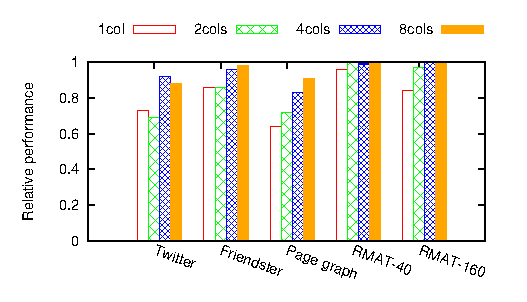
\includegraphics[scale=1]{SpMM_figs/spmm_im_vs_sem.eps}
		\vspace{-5pt}
		\caption{The runtime performance of SEM-SpMM, normalized to IM-SpMM
		for the dense matrix with the same number of columns.}
		\label{perf:spmm_comp}
	\end{subfigure}
	\begin{subfigure}[b]{0.5\textwidth}
		\centering
		\vspace{5pt}
		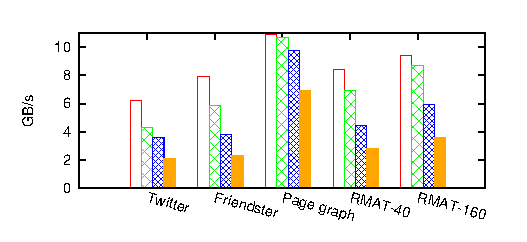
\includegraphics[scale=1]{SpMM_figs/spmm_IO.eps}
		\vspace{-5pt}
		\caption{The I/O throughput generated by SEM-SpMM.}
		\label{perf:spmm_IO}
	\end{subfigure}
	\vspace{3pt}
	\caption{The performance and the I/O throughput of SEM-SpMM with dense
	matrices of different numbers of columns.}
	\label{perf:spmm_IM_vs_SEM}
\end{figure}

We compare the performance of SEM-SpMM with IM-SpMM to investigate
the performance penalty of scaling SpMM with SSDs. In this case, the dense
matrices have a small number of columns and are stored in memory. 

There is only a small performance penalty for semi-external memory (Figure
\ref{perf:spmm_comp}). The performance gap between IM-SpMM and SEM-SpMM
is affected by randomness of vertex connection. The gap is smaller if
vertex connection in a graph is more random. The Page graph is relatively
well clustered, so SpMM on this graph is less CPU-bound than others.
Even for the Page graph, SEM-SpMM gets 65\% performance of IM-SpMM.
The other factor of affecting the performance gap is the number of columns
in the dense matrices. The gap gets smaller as the number of columns in
the dense matrices increases.

We further measure the average I/O throughput generated by SEM-SpMM to indicate
the bottleneck of the system (Figure \ref{perf:spmm_IO}). SpMV on the Page
graph saturates the I/O bandwidth of SSDs and is clearly bottlenecked by I/O.
SpMV on other graphs (except Twitter) also generates high I/O throughput,
which consumes memory bandwidth and potentially interferes with random memory
access in SpMV. SEM-SpMV on the Twitter graph takes about 0.5 second to
complete and,
thus, startup overhead has significant impact on the average I/O throughput.
As the number of columns in the dense matrix increases, SpMM becomes more CPU
bound. For all graphs, SEM-SpMM requires a very small number of columns to
become CPU-bound and achieve close to 100\% performance of IM-SpMM.

\subsection{SEM-SpMM vs. other in-memory SpMM}
In this section, we compare SEM-SpMM with the Intel MKL and Trilinos Tpetra
implementations. Intel MKL runs on shared-memory machines. Trilinos Tpetra can run in
both shared memory and distributed memory, so we measure its performance in
our 48-core NUMA machine as well as an EC2 cluster. We run Tpetra in the largest
EC2 instances r3.8xlarge, where each has 16 physical CPU cores and 244GB of RAM
and is optimized for memory-intensive applications. The EC2 instances are
connected with 10Gbps network in the same placement group.

\begin{figure}
	\footnotesize
	\centering
	\begin{subfigure}[b]{0.5\textwidth}
		\centering
		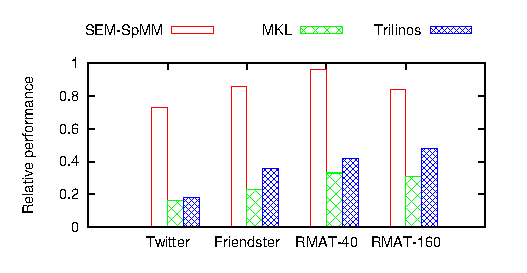
\includegraphics[scale=1]{SpMM_figs/SpMV-awesomer.eps}
		\vspace{-5pt}
		\caption{SpMV}
		\label{perf:spmv}
	\end{subfigure}
	\begin{subfigure}[b]{0.5\textwidth}
		\centering
		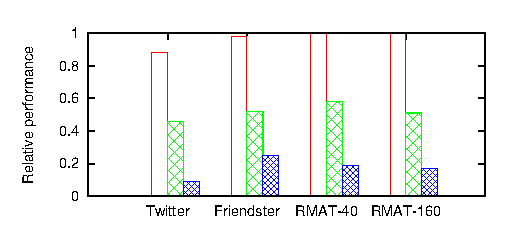
\includegraphics[scale=1]{SpMM_figs/SpMM-awesomer.eps}
		\vspace{-5pt}
		\caption{SpMM with a dense matrix of 8 columns.}
		\label{perf:spmm8}
	\end{subfigure}
	\vspace{3pt}
	\caption{The performance of different sparse matrix multiplication
		implementations on the 48-core machine normalized to IM-SpMM for
	the same graphs.}
	\label{perf:spmm}
\end{figure}

Our SEM-SpMM significantly outperforms Intel MKL and Trilinos Tpetra on the natural
graphs on our NUMA machine (Figure \ref{perf:spmm}). In this case, we compare
performance of our SEM-SpMM with Intel MKL and Trilinos Tpetra for both sparse matrix
vector multiplication (SpMV) and sparse matrix dense matrix multiplication (SpMM).
The Tpetra implementation is optimized for SpMV. Our SEM-SpMM still constantly
outperforms Tpetra by a factor of $2-3$ even for SpMV. The MKL implementation has
better optimizations for SpMM than Trilinos Tpetra. Our SEM-SpMM is still almost
twice as fast as MKL in SpMM with a dense matrix of eight columns. There are multiple
reasons that our SEM-SpMM outperforms the ones in MKL and Tpetra. Neither MKL nor
Tpetra balance loads dynamically. In addition, they store a sparse matrix in CSC
or CSR format, which leads to many CPU cache misses. Because the SpMM in Tpetra
is implemented with MPI, it has additional memory copy overhead to exchange
partitions of the input dense matrix among processes.

SEM-SpMM only consumes a small fraction of memory compared with IM-SpMM and
other SpMM implementations (Figure \ref{perf:spmm_mem}). SEM-SpMM consumes
memory for the input dense matrix as well as per-thread local memory buffers
for the sparse matrix and the output dense matrix. When we use 48 threads for
SpMM, the memory used by local memory buffers in each thread is significant
but is relatively constant for different graph sizes. We only show the memory
consumption on one of the large graphs RMAT-160 in Figure \ref{perf:spmm_mem}.
Despite considerable memory used by local memory buffers, SEM-SpMM uses about
one tenth of the memory
used by IM-SpMM. We also observe that IM-SpMM consumes much less memory than
MKL and Tpetra owing to its compact format for sparse matrices.

\begin{figure}
	\begin{center}
		\footnotesize
		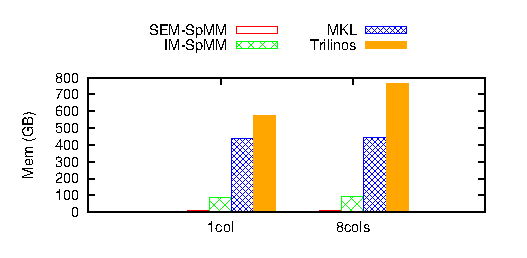
\includegraphics[scale=1]{SpMM_figs/SpMM-mem.eps}
		\caption{Memory consumption of different SpMM implementations on
		RMAT-160.}
		\label{perf:spmm_mem}
	\end{center}
\end{figure}

\begin{figure}
	\footnotesize
	\centering
	\begin{subfigure}[b]{0.5\textwidth}
		\centering
		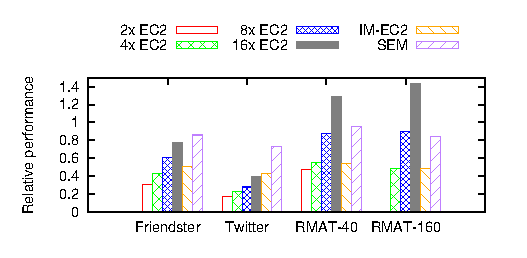
\includegraphics[scale=1]{SpMM_figs/SpMV-EC2.eps}
		\vspace{-5pt}
		\caption{SpMV}
		\label{perf:ec2:spmv}
	\end{subfigure}
	\begin{subfigure}[b]{0.5\textwidth}
		\centering
		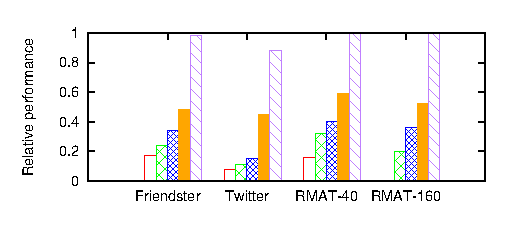
\includegraphics[scale=1]{SpMM_figs/SpMM-EC2.eps}
		\vspace{-5pt}
		\caption{SpMM with a dense matrix of 8 columns.}
		\label{perf:ec2:spmm8}
	\end{subfigure}
	\vspace{3pt}
	\caption{The performance of SEM-SpMM on our 48-core machine (SEM) and
		Trilinos Tpetra on EC2 clusters (2xEC2, 4xEC2 and 8xEC2), normalized to
		IM-SpMM on our 48-core machine for the same graphs. We also show
		the performance of IM-SpMM on
	one of the EC2 instance (IM-EC2) where Trilinos Tpetra runs.}
	\label{perf:ec2}
\end{figure}

Our SpMM implementation uses much less computation resources to achieve
comparable performance and, in many cases, outperforms Trilinos Tpetra that
runs in the Amazon cloud, especially on real-world graphs (Figure
\ref{perf:ec2}). In this experiment, we run our SpMM implementation on both
our NUMA machine with 48 CPU cores
and one of the EC2 machines with 16 CPU cores. Owing to the compact format
for a sparse matrix, our SpMM implementation can run on all of the graphs
in memory on an EC2 instance. When Tpetra runs on 8 EC2 instances, it has
2.5 times as many CPU cores as our NUMA machine. Tpetra is not
able to run SpMV on RMAT-160 on two EC2 nodes. Even though an EC2 instance
has only 16 physical CPU cores, our IM-SpMM on an EC2 instance achieves around
half of the performance of our IM-SpMM on our NUMA machine. In contrast,
Trilinos Tpetra uses many more computation resources and still barely reaches
the same performance as our IM-SpMM and SEM-SpMM on our NUMA machine. One of
the main reasons that our SpMM implementation performs much
better on real-world graphs is that these graphs are more likely to cause
load imbalance. Our SpMM implementation balances load much better than
distributed implementations that partition data.

\subsection{SEM-SpMM with a large input dense matrix}

We further measure the performance of SEM-SpMM with a large input dense matrix,
in which neither the sparse matrix nor the dense matrices can fit in memory.
In this experiment, we measure the performance of multiplying a sparse matrix
with a dense matrix of 32 columns and the input dense matrix is stored on SSDs
initially. We study the impact of memory size on the performance of SEM-SpMM
by artificially varying the number of columns that can fit in memory. SEM-SpMM
accesses
the sparse matrix with direct I/O and, thus, varying the number of columns
in the dense matrix that fit in memory does not affect data access to the
sparse matrix. In each run, we need to load the input dense matrix from
SSDs and stream the output dense matrix to SSDs. We do not show the result on
the Page graph because the dense matrix with 32 columns for the Page graph
cannot fit in memory.

\begin{figure}
	\begin{center}
		\footnotesize
		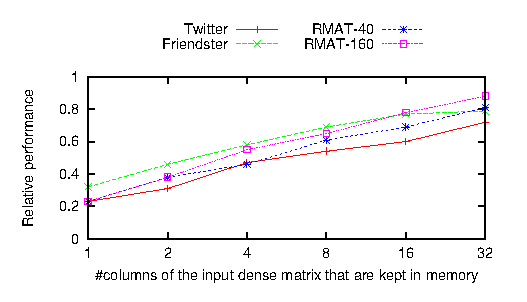
\includegraphics[scale=1]{SpMM_figs/spmm-32cols.eps}
		\caption{The performance of SEM-SpMM with a dense matrix of 32 columns
			relative to IM-SpMM, when the number of columns of the input dense
		matrix kept in memory varies.}
		\label{perf:spmm32}
	\end{center}
\end{figure}

As more columns in the input dense matrix can fit in memory, the performance
of SEM-SpMM constantly increases (Figure \ref{perf:spmm32}). When the memory
can fit over four columns of the input dense matrix, SEM-SpMM gets over 50\%
of the performance of IM-SpMM. Even when only one column of the input dense
matrix can fit in memory, SEM-SpMM still gets 25\% of the in-memory performance.
When the entire input dense matrix can fit in memory, we get about 80\% of
the in-memory performance.

\begin{figure}
	\begin{center}
		\footnotesize
		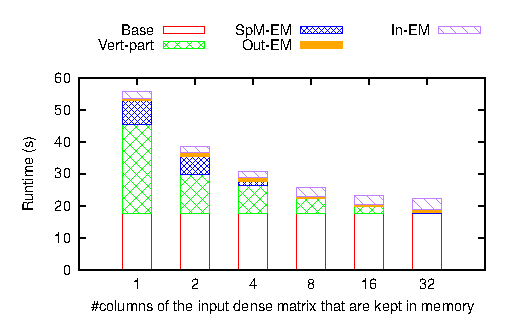
\includegraphics[scale=1]{SpMM_figs/spmm-32cols-overhead.eps}
		\caption{The overhead breakdown of SEM-SpMM on the Friendster
			graph with a dense matrix of 32 columns when the number
		of columns in the input dense matrix kept in memory varies. }
		\label{perf:spmm32_over}
	\end{center}
\end{figure}

Two main factors lead to performance loss in SEM-SpMM when the input dense matrix
cannot fit in memory. We illustrate the contribution of four potential overheads
in SEM-SpMM on the Friendster graph (Figure \ref{perf:spmm32_over}). The main
performance loss comes from the loss of data locality in SpMM caused by
vertical partitioning of the input dense matrix (Vert-part). Partitioning
the dense matrix into one-column matrices contributes 60\% of performance loss.
It drops quickly when the vertical
partition size increases. Keeping the sparse matrix on SSDs (SpM-EM)
also contributes some performance loss when the dense matrix is partitioned
into small matrices. The overhead almost goes away when more than four columns
of the dense matrix can fit in memory. The overhead of streaming the output dense
matrix to SSDs (Out-EM) and reading the input dense matrix to memory (In-EM)
is less significant and remains the same for different memory sizes.

\subsection{Optimizations on sparse matrix multiplication}
Accelerating SEM-SpMM requires both computation and I/O optimizations.
We first evaluate the effectiveness of computation optimizations by deploying
them on IM-SpMM. We further show the effectiveness of I/O optimizations by
deploying them on SEM-SpMM with all computation optimizations.

Here we illustrate the most significant computation optimizations from Section
\ref{sec:spmm}. We start with an in-memory implementation that
performs sparse matrix multiplication on a sparse matrix in the CSR format
and apply the optimizations incrementally in the following order:
\begin{itemize} \itemsep1pt \parskip0pt \parsep0pt
	\item dispatch partitions of a sparse matrix to threads dynamically
		to balance load (\textit{Load balance}),
	\item partition dense matrices for NUMA (\textit{NUMA}),
	\item organize the non-zero entries in a sparse matrix into tiles to
		increase CPU cache hits (\textit{Cache blocking}),
	\item use CPU vectorization instructions to accelerate arithmetic
		computation (\textit{Vec}),
\end{itemize}

All of these optimizations have positive effects on sparse matrix
multiplication and all optimizations together speed up SpMM by $3-5$ times
(Figure \ref{perf:spmm_opt}). The degree of effectiveness
varies between different graphs and different numbers of columns in
the dense matrices. The largest performance boost is from cache blocking,
especially for SpMV. This is expected because these graphs have near-random
vertex connection, which leads many random memory access in sparse matrix
multiplication. Cache blocking significantly increases CPU cache hits to reduce
random memory access. CPU vectorization is only effective on SpMM because
it optimizes computation on a row of the dense matrix.
%For example, the NUMA optimization is more effective when
%the dense matrices have more columns because more columns in the dense
%matrices require more memory bandwidth. Cache blocking is very effective when
%the dense matrices have fewer columns because it can effectively increase CPU
%cache hits. When there are more columns in the dense matrices, data locality
%improves and the effectiveness of cache blocking becomes less noticeable.
%When there are too many columns, the rows from the input and output matrices
%can no longer be in the CPU cache.
With all optimizations, we have a fast in-memory implementation for both
sparse matrix vector multiplication and sparse matrix dense matrix multiplication.

\begin{figure}
	\begin{center}
		\footnotesize
		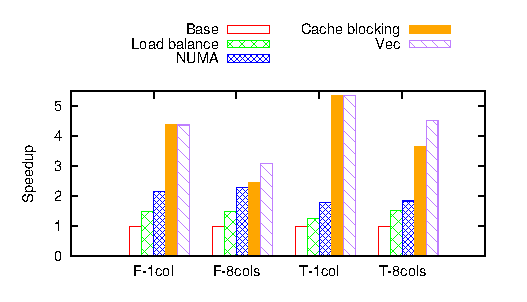
\includegraphics[scale=1]{SpMM_figs/SpMM_optimize.eps}
		\caption{The speedup of each computation optimization for SpMV and SpMM
			on the Friendster (F) and Twitter (T) graph. The input dense matrix
		in SpMM has 8 columns.}
		\label{perf:spmm_opt}
	\end{center}
\end{figure}

We evaluate I/O optimizations on SEM-SpMV against a base implementation that
has all of the computation optimizations and use doubly compressed sparse row
format (DCSR) to store tiles of a sparse matrix. We illustrate their
effectiveness on the Friendster graph and the Page graph. The first one
represents a graph that is not well clustered; the other one is clustered with
domain names. We apply the I/O optimizations in the following order:
\begin{itemize} \itemsep1pt \parskip0pt \parsep0pt
	\item use SCSR to reduce data read from SSDs (SCSR),
	\item reduce memory allocation overhead for I/O with per-thread buffer
		pools (\textit{buf-pool}),
	\item reduce the number of thread context switches for I/O accesses with I/O
		polling (\textit{IO-poll}),
\end{itemize}

\begin{figure}
	\begin{center}
		\footnotesize
		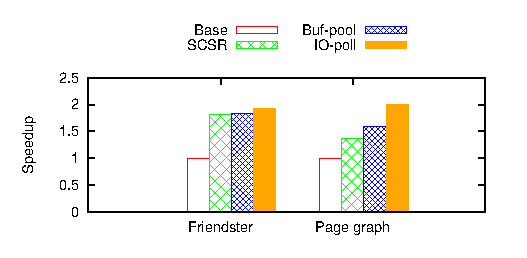
\includegraphics[scale=1]{SpMM_figs/io_opts.eps}
		\caption{The speedup of I/O optimizations for SpMV on the Friendster
		graph and the Page graph.}
		\label{perf:spmm_opt_io}
	\end{center}
\end{figure}

The I/O optimizations lead to substantial speedup over the base implementation,
but behave very differently on these two graphs (Figure \ref{perf:spmm_opt_io}).
On the unclustered graph (Friendster), SCSR requires a much smaller storage size
than DCSR (Figure \ref{fig:storage}) and thus achieves significant
speedup. The Page graph, on the other hand, is well clustered and DCSR already
achieves a small storage size. SCSR further reduces the storage size, but is
less significant. SpMV on the Page graph has less random memory access and is
I/O-bound even on a large SSD array. \textit{Buf-pool} and \textit{IO-poll}
increases I/O throughput and, thus, improves performance. In contrast, SEM-SpMV
with the Friendster graph in the SCSR format already achieves almost 80\% of
IM-SpMV and, thus, further I/O optimizations have less noticeable speedup.

\subsection{Performance of the applications}

We evaluate the performance of our implementations of the applications in
Section \ref{sec:spmm:apps}. We show the effectiveness of additional memory for
these applications and compare their performance with state-of-the-art
implementations.

\subsubsection{PageRank}
We evaluate the performance of our SpMM-based PageRank implementation
(SpMM-PageRank). This implementation requires the input vector to be in memory,
but it is optional to keep the output vector and the degree vector in memory.
PageRank is a benchmarking graph algorithm implemented by many graph processing
frameworks. We compare the performance of SpMM-PageRank with state-of-the-art
implementations in FlashGraph \cite{flashgraph}, a semi-external memory graph
engine, and GraphLab Create, the next generation of PowerGraph \cite{powergraph}.
The PageRank implementation in FlashGraph computes
approximate PageRank values while SpMM-PageRank and GraphLab Create compute
exact PageRank values. We run GraphLab Create completely in memory and
FlashGraph in semi-external memory. GraphLab Create is not able to compute
PageRank on the Page graph. We use FlashGraph v0.3 and a trial version of
GraphLab Create v1.9.

SpMM-PageRank in memory and in semi-external memory both significantly outperform
the implementations in FlashGraph and GraphLab Create (Figure \ref{perf:pagerank}).
Our SpMM is highly optimized for both CPU
and I/O. Even though SpMM-PageRank performs more computation than FlashGraph,
it performs the computation much more efficiently and
reads less data from SSDs than FlashGraph. SpMM-PageRank and the implementation
in GraphLab create performs the same computation, but SpMM-PageRank
performs the computation much more efficiently.

The experiment results also show that keeping more vectors in memory has modest
performance improvement for SpMM-PageRank. As such, SpMM-PageRank only needs
to keep one vector in memory, which results in very small memory consumption.

\begin{figure}
	\begin{center}
		\footnotesize
		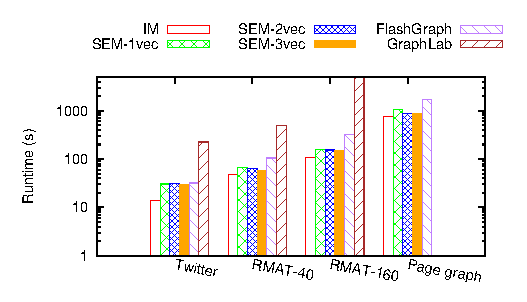
\includegraphics[scale=1]{SpMM_figs/pagerank.eps}
		\caption{The runtime of SpMM-PageRank in 30 iterations. The SEM
			implementation keeps different numbers of vectors in memory
			(SEM-1vec, SEC-2vec, SEM-3vec). We compare them with
		the implementations in FlashGraph and GraphLab Create.}
		\label{perf:pagerank}
	\end{center}
\end{figure}

\subsubsection{Eigensolver}

We evaluate the performance of our SEM KrylovSchur eigensolver and compare
its performance
with our in-memory eigensolver and the Trilinos KrylovSchur eigensolver.
Usually, spectral analysis only requires a very small number of
eigenvalues, so we compute eight eigenvalues in this experiment. We run
the eigensolvers on the smaller undirected graphs
in Table \ref{graphs}. To evaluate the scalability of the SEM eigensolver,
we compute singular value decomposition (SVD) on the Page graph. Among all of
the eigensolvers, only our SEM eigensolver is able to compute eigenvalues
on the Page graph.

\begin{figure}
	\begin{center}
		\footnotesize
		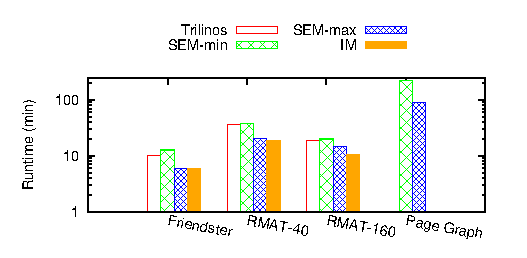
\includegraphics[scale=1]{SpMM_figs/eigen-runtime-8ev.eps}
		\caption{The runtime of our SEM KrylovSchur, our in-memory eigensolver
			and the Trilinos eigensolvers when computing eight
			eigenvalues. SEM-min keeps the entire vector subspace on SSDs and
		SEM-max keeps the entire vector subspace in memory.}
		\label{fig:eigen}
	\end{center}
\end{figure}

For computing 8 eigenvalues, our SEM eigensolver achieves performance
comparable to our in-memory eigensolver and the Trilinos eigensolver
and can scale to very large graphs (Figure \ref{fig:eigen}).
Unlike PageRank, an eigensolver has many more vector or dense matrix operations.
As such, the memory size has noticeable impact on performance.
For the setting with the minimum memory consumption, it has at least 45\%
performance of our in-memory eigensolver; when keeping the entire subspace
in memory, it has almost the same performance as our in-memory eigensolver.

\subsubsection{NMF}
We evaluate the performance of our NMF implementation (SEM-NMF) on the directed
graphs in Table \ref{graphs}. The dense matrices for NMF can be as large as
the sparse matrix. As such, we experiment with the effect of the memory size on
the performance of SEM-NMF by varying the number of columns in memory from
the dense matrices. We also compare the performance of SEM-NMF with
a high-performance NMF implementation SmallK \cite{SmallK}, built on top of
the numeric library Elemental \cite{elemental}. We factorize
each of the graphs into two $n \times k$ non-negative dense matrices and
we use $k=16$ because $16$ is the largest $k$ that SmallK supports for
the graphs in Table \ref{graphs}. We use SmallK v1.6 and Elemental v0.85.

\begin{figure}
	\begin{center}
		\footnotesize
		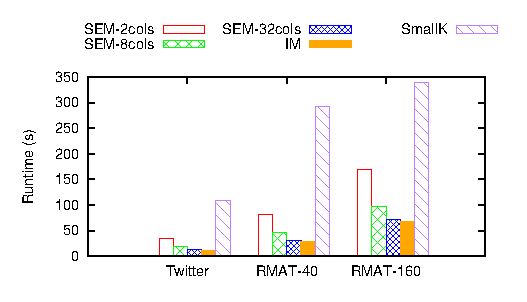
\includegraphics[scale=1]{SpMM_figs/NMF.eps}
		\caption{The runtime per iteration of SEM-NMF on directed graphs.
			We vary the number of columns in the dense matrices that are kept
			in memory to evaluate effect of the memory size on the performance
		of SEM-NMF.}
		\label{perf:NMF}
	\end{center}
\end{figure}

We significantly improve the performance of SEM-NMF by keeping more columns
of the input dense matrix in memory (Figure \ref{perf:NMF}). The performance
improvement is more significant when the number of columns that fit in memory
is small. When we keep eight columns of the input dense matrix in memory,
SEM-NMF achieves over 60\% of the performance of the in-memory implementation.

SEM-NMF significantly outperforms other NMF implementations in the literature.
SmallK is the closest competitor. We run the same NMF algorithm in SmallK and
SEM-NMF outperforms SmallK by a large factor on all graphs (Figure
\ref{perf:NMF}). There are many MapReduce implementations in
the literature \cite{Liao14, Yin14, Liu10}. They run on sparse
matrices with tens of millions of non-zero entries but generally take
one or two orders of magnitude more time than our SEM-NMF on the sparse matrices
with billions of non-zero entries.
